\documentclass[14pt]{extarticle}
\usepackage[T1]{fontenc}

\usepackage[english]{babel}

\usepackage[a4paper, margin=2cm]{geometry}
\usepackage[parfill]{parskip}

\usepackage{amsmath}
\usepackage{amsfonts}
\usepackage{amsthm}

\usepackage{graphicx}
\usepackage{float}

\usepackage{array}
\usepackage{booktabs}

\usepackage{hyperref}
\hypersetup{colorlinks=true, urlcolor=blue}
\urlstyle{same}

\usepackage[outputdir=out]{minted}
\usemintedstyle{vs}

\begin{document}
    \author{Elia Perantoni}
    \title{ Machine Learning Project \\
        \large Classifying human activities \\
        (Project \#3) }
    \maketitle

    \section{Introduction}
    We want to build a machine learning classifier on the \emph{Human Activity
    Recognition with Smartphones} dataset, available at the following
    \href{https://www.kaggle.com/datasets/uciml/human-activity-recognition-with-smartphones}{link}.

    The data has been gathered by having $30$ subjects performing $6$ different
    physical activities (laying, standing, sitting, walking, walking upstairs
    and walking downstairs) while a waist-mounted smartphone records
    accelerometer and gyroscope state.

    Each sample originally consisted of $3$-axis linear acceleration and
    $3$-axis angular velocity but has been feature-engineered, by the authors,
    to a grand total of $561$ features, obtained by filtering, mixing and
    matching the primitive ones.

    The dataset is already split in $7352$ training samples and $2947$ testing
    samples.

    \section{Class Encoding}
    To make the rest of the code easier, we encode the labels (given as strings)
    to integers using the \mintinline{python}{ClassMapper} class.

    \begin{minted}{python}
# train_y is ["WALKING", "STANDING", "WALKING", ... ]
cm = ClassMapper(train_y)
train_y = cm.transform(train_y)
# train_y is [0, 1, 0, ... ]
    \end{minted}

    \section{PCA}
    We start by performing \emph{Principal Component Analysis} to reduce the
    number of features and make classification easier.

    The \mintinline{python}{pca} function takes in a $n\times d$ matrix ($n$ is
    the number of samples and $d$ is the number of features), a
    \mintinline{python}{retain} coefficient that indicates how many axes the
    data should be projected on, and returns a Python function that performs the
    dimensionality reduction.

    \begin{minted}{python}
pca_reduce = pca(train_X, retain=0.3, verbose=True)
train_X = pca_reduce(train_X)
    \end{minted}

    \mintinline{python}{retain=0.3} means that the samples will be projected on
    $0.3\cdot d$ axes. In our case, the samples are scaled from $561$ features
    down to $168$.

    \begin{figure}[H]
        \centering
        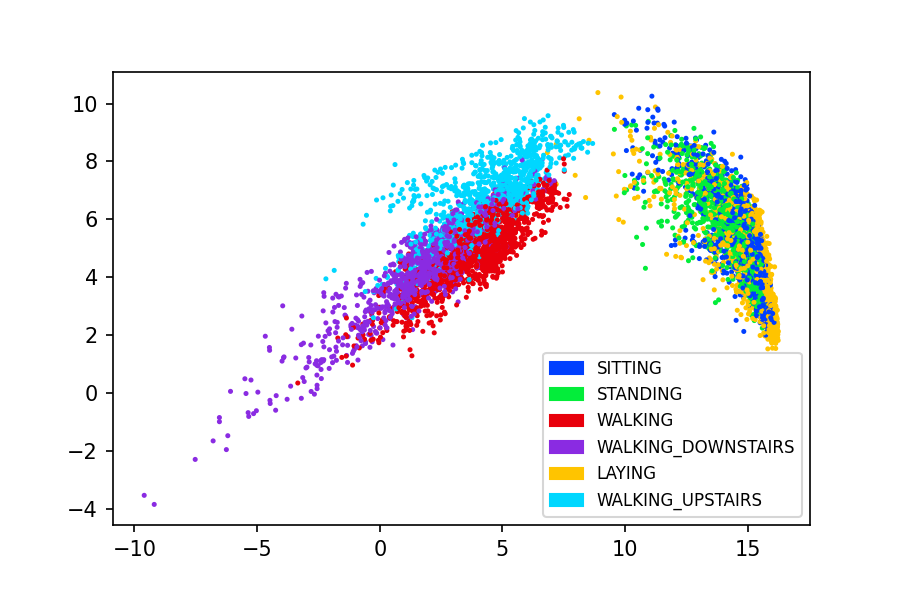
\includegraphics[width=0.8\textwidth]{img/pca_3.png}
        \caption{PCA processed data projected on first two features}
    \end{figure}

    \section{LDA}
    To make classification even easier, we apply \emph{Linear Discriminant
    Analysis} to transform the data such that classes are tightly packed and
    distant from each other. Since we have $k=6$ classes, we will be projecting
    on $k-1=5$ axes.

    The implementation is functionally the same as \emph{PCA}: a function takes
    in some data and produces a function that performs the \emph{LDA}
    dimensionality reduction. The only differences are that we no longer need a
    \mintinline{python}{retain} argument but now require the labels
    \mintinline{python}{train_y}.

    \begin{minted}{python}
lda_reduce = lda(train_X, train_y, verbose=True)
train_X = lda_reduce(train_X)
    \end{minted}

    \begin{figure}[H]
        \centering
        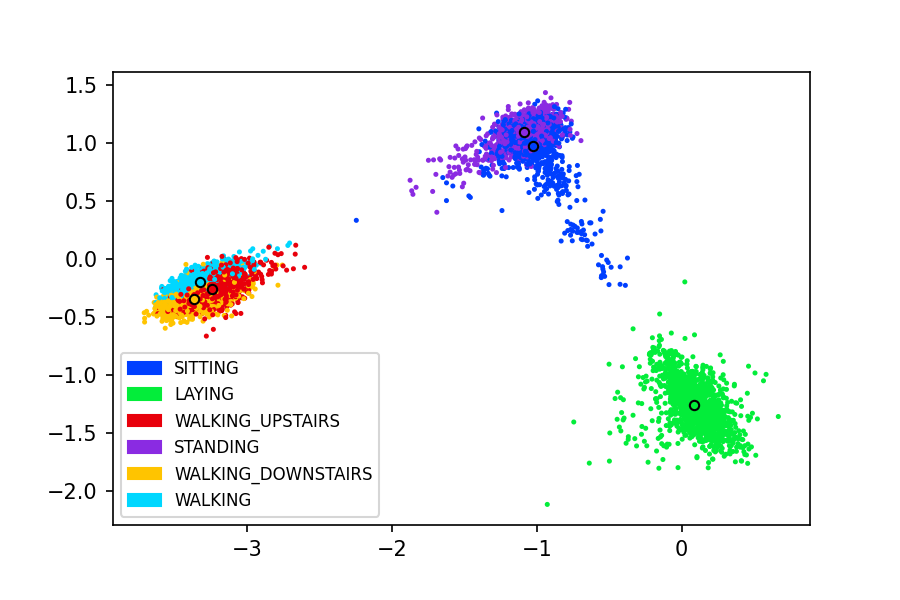
\includegraphics[width=0.8\textwidth]{img/lda_1.png}
        \caption{PCA+LDA processed data projected on first two features}
    \end{figure}

    \section{Classification}
    Now that we have $7352$ samples of $5$ features each, we can start training
    a classification system.

    I chose to go down the naive Bayesian route. There are $k=6$ multivariate
    Gaussian distributions, one for each class, that attempt to enclose the
    regions of $\mathbb{R}^5$ in which the samples of each class occur. The
    Gaussian distributions are trained simply by partitioning the training
    samples by class and, for each partition, computing the mean $\boldsymbol{\mu}$ and
    covariance matrix $\boldsymbol{\Sigma}$. Although the classes are quite
    evenly distributed, the prior probability $p(\omega_i)=\frac{|X\ \cap\ \omega_i|}{|X|}$
    is also computed.

    To make a new prediction on an unseen sample $\boldsymbol{x}$, simply take
    the class whose Gaussian distribution returns the greatest posterior probability.

    \[
      \operatorname*{argmax}_{\omega_i} p(\omega_i\mid\boldsymbol{x}) =
      \frac{p(\boldsymbol{x}\mid\omega_i)\cdot p(\omega_i)}{p(\boldsymbol{x})} =
      p(\boldsymbol{x}\mid\omega_i)\cdot p(\omega_i)
    \]

    The evidence probability $p(\boldsymbol{x})$ can be ignored because it only
    normalizes the posteriors, the winning class would still be the same.

    \section{Results}
    Our simple classifier achieves an accuracy of $0.9613$. Compare this with
    other, more sophisticated, classifiers (from the \emph{SciKit-Learn}
    library).

    \begin{center}
    \begin{tabular}{cc}
        Algorithm & Accuracy \\
        \midrule
        Random Forest & $0.9636$ \\
        Naive Bayes \textit{(ours)} & $0.9613$ \\
        SVM & $0.9613$ \\
        Multi-Layer Perceptron Neural Network & $0.9613$ \\
        $K$-Nearest & $0.9606$
    \end{tabular}
    \end{center}
\end{document}